% !TeX root = ../../main.tex
\subsection{Dialog}

Por meio do dialog foi possível reunir em um único menu as principais funcionalidades de configuração e monitoramento do sistema, permitindo que usuários realizem tarefas administrativas sem a necessidade de memorizar comandos do sistema operacional.

A Figura \ref{fig:dialog1} apresenta o menu principal da aplicação, no qual o usuário seleciona a máquina virtual que deseja configurar. Essa etapa organiza o gerenciamento do ambiente, permitindo que cada máquina seja administrada individualmente.

\begin{figure}[H]
    \centering
    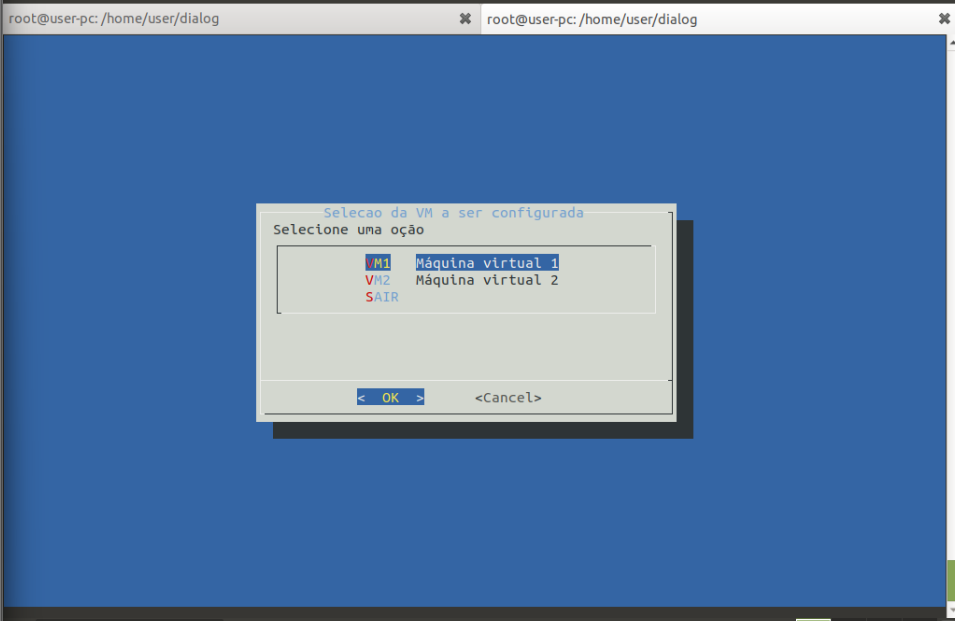
\includegraphics[width=1\linewidth]{fig/dialog/dialog1.png}
    \caption{Menu principal}
    \label{fig:dialog1}
\end{figure}

A partir da seleção da máquina virtual, é exibido o menu de controle apresentado na Figura \ref{fig:dialog2}. Nesse menu encontram-se disponíveis as principais operações do sistema, como configuração automática e manual das interfaces de rede, gerenciamento de processos, visualização das configurações do sistema e execução dos testes utilizando o Iperf.

\begin{figure}[H]
    \centering
    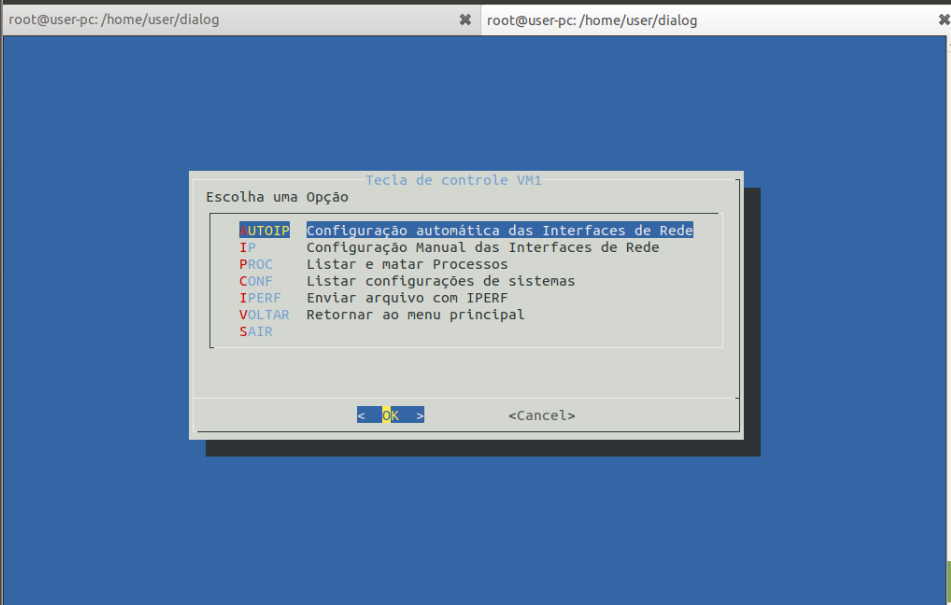
\includegraphics[width=1\linewidth]{fig/dialog/dialog2.png}
    \caption{Menu controle da VM - AutoIP}
    \label{fig:dialog2}
\end{figure}


A configuração automática das interfaces de rede é realizada pela opção \textit{AutoIP}. Conforme ilustrado na Figura \ref{fig:dialog3}, o usuário informa os parâmetros necessários, como endereço IP, máscara de rede, interface de rede, gateway e a senha do computador. Após a confirmação, a aplicação realiza automaticamente as configurações correspondentes no sistema operacional, reduzindo a necessidade de edição manual dos arquivos de configuração.

\begin{figure}[H]
    \centering
    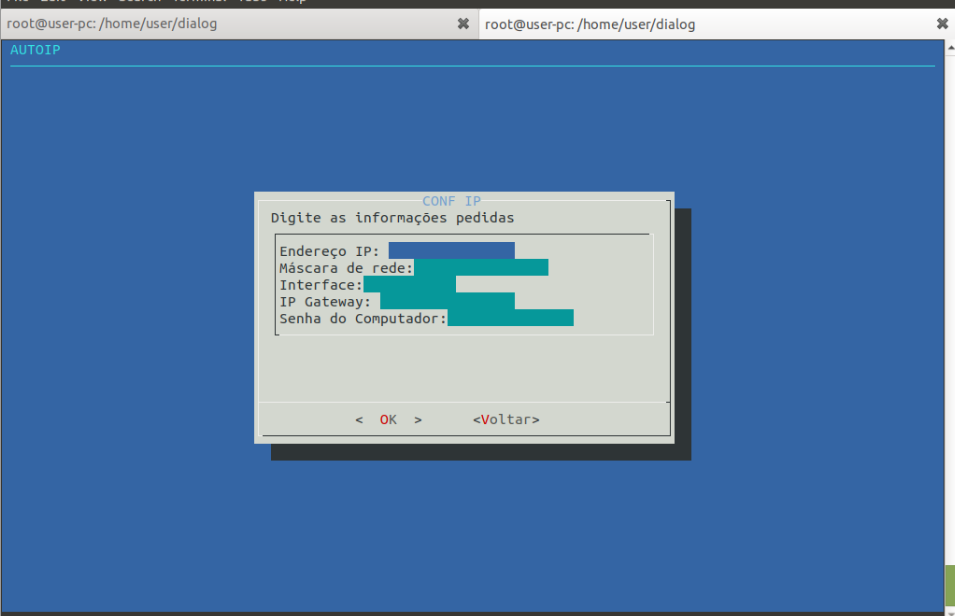
\includegraphics[width=1\linewidth]{fig/dialog/dialog3.png}
    \caption{Configuração auto IP}
    \label{fig:dialog3}
\end{figure}

Caso seja necessária uma configuração mais detalhada, a opção de configuração manual pode ser utilizada. A Figura \ref{fig:dialog4} apresenta novamente o menu principal de controle da máquina virtual, destacando a opção responsável pelo acesso às configurações individuais das interfaces de rede.


\begin{figure}[H]
    \centering
    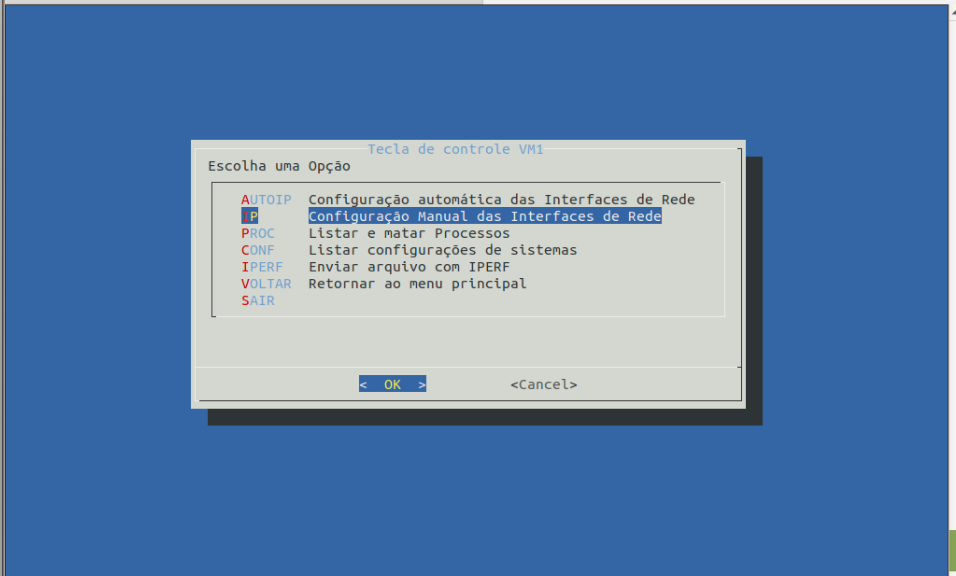
\includegraphics[width=1\linewidth]{fig/dialog/dialog4.png}
    \caption{Menu controle da VM - Configuração manual das interfaces}
    \label{fig:dialog4}
\end{figure}

Ao selecionar essa funcionalidade, é exibido o submenu ilustrado na Figura \ref{fig:dialog5}, no qual o usuário pode configurar separadamente o gateway padrão e as informações de DNS do sistema. Essa divisão torna a interface mais organizada e permite alterar apenas os parâmetros desejados, sem interferir nas demais configurações da máquina virtual.


\begin{figure}[H]
    \centering
    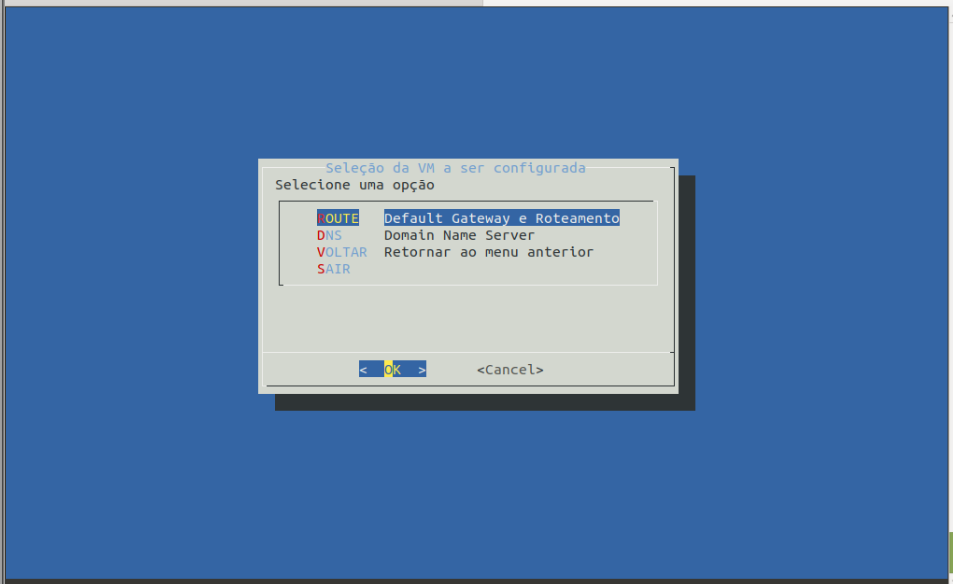
\includegraphics[width=1\linewidth]{fig/dialog/dialog5.png}
    \caption{Menu para seleção de configuração de gateway, DNS}
    \label{fig:dialog5}
\end{figure}

A Figura \ref{fig:dialog6} apresenta o resultado da consulta à tabela de roteamento da máquina virtual. Nessa tela são exibidas as rotas atualmente configuradas, incluindo o gateway padrão e as redes diretamente conectadas. Essa funcionalidade permite verificar rapidamente se as alterações realizadas na configuração de rede foram aplicadas corretamente, facilitando a identificação de inconsistências na comunicação entre os dispositivos.


\begin{figure}[H]
    \centering
    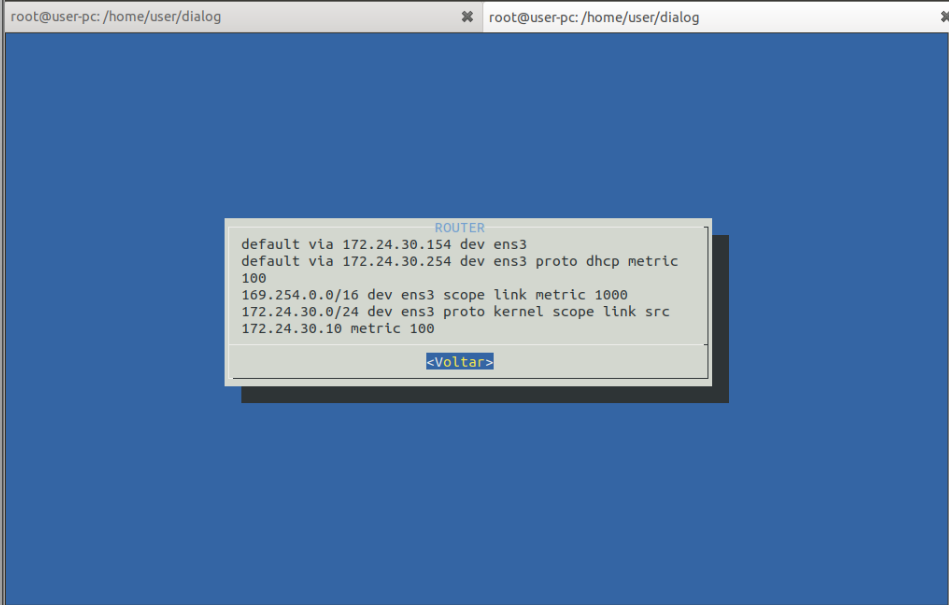
\includegraphics[width=1\linewidth]{fig/dialog/dialog6.png}
    \caption{Rotas configuradas}
    \label{fig:dialog6}
\end{figure}

A configuração dos servidores DNS é realizada por meio da interface apresentada na Figura \ref{fig:dialog7}. O usuário informa os endereços do servidor DNS primário e secundário, além da senha necessária para a execução das alterações. Após a confirmação, a aplicação atualiza automaticamente os arquivos de configuração do sistema, dispensando a edição manual.


\begin{figure}[H]
    \centering
    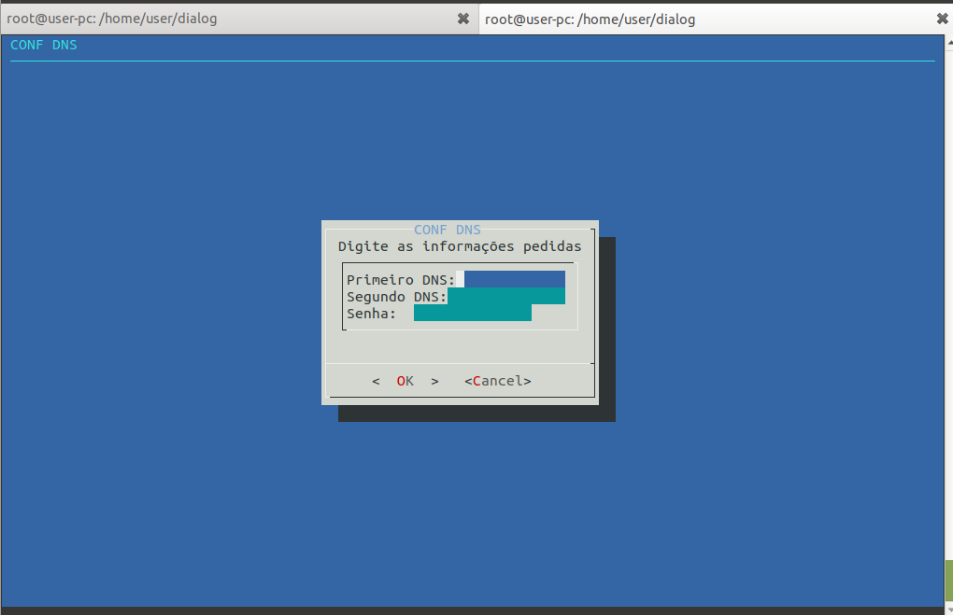
\includegraphics[width=1\linewidth]{fig/dialog/dialog7.png}
    \caption{Menu para configuração do DNS}
    \label{fig:dialog7}
\end{figure}


Durante a aplicação das configurações, é exibida a janela ilustrada na Figura \ref{fig:dialog8}. Essa tela informa ao usuário que as modificações estão sendo executadas, fornecendo um retorno visual sobre o andamento da operação e evitando a interrupção do processo antes de sua conclusão.


\begin{figure}[H]
    \centering
    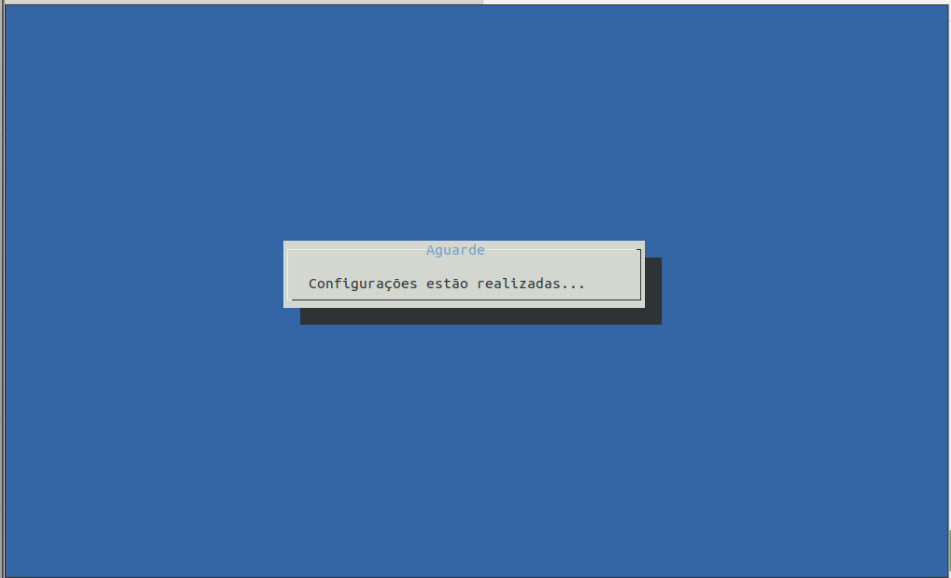
\includegraphics[width=1\linewidth]{fig/dialog/dialog8.png}
    \caption{Menu de configurações sendo realizada}
    \label{fig:dialog8}
\end{figure}


Além das funcionalidades relacionadas à configuração de rede, a interface disponibiliza recursos para administração de processos em execução. A Figura \ref{fig:dialog9} apresenta a listagem dos processos ativos na máquina virtual, contendo informações como o identificador do processo (PID), terminal associado e comando executado. Essa funcionalidade possibilita ao administrador acompanhar rapidamente o estado atual do sistema.


\begin{figure}[H]
    \centering
    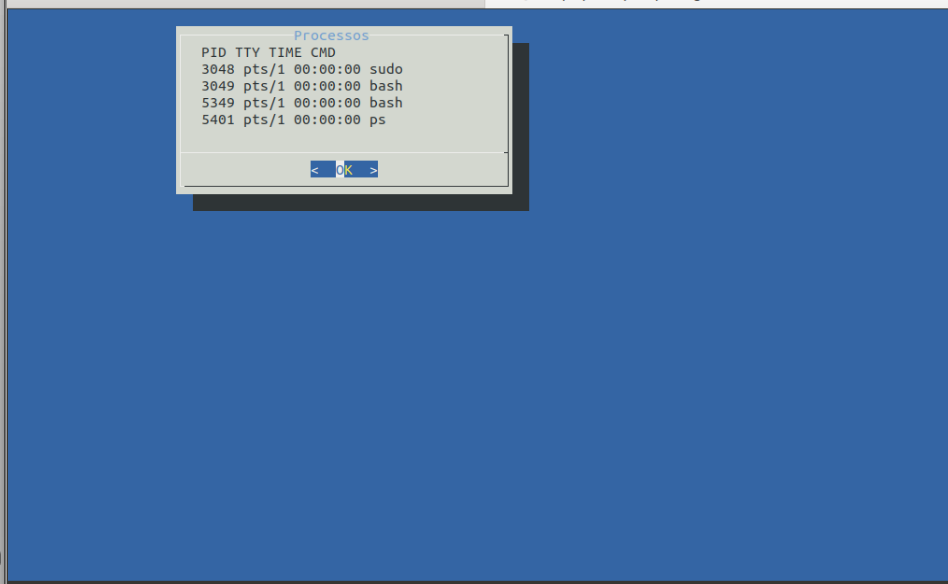
\includegraphics[width=1\linewidth]{fig/dialog/dialog9.png}
    \caption{Lista de processos}
    \label{fig:dialog9}
\end{figure}

Após a exibição da lista de processos, a aplicação oferece a opção de finalizar algum processo em execução, conforme apresentado na Figura \ref{fig:dialog10}. Antes da execução da operação, uma janela de confirmação é exibida ao usuário, reduzindo a possibilidade de encerramento acidental de processos importantes e proporcionando maior segurança durante a administração do ambiente.


\begin{figure}[H]
    \centering
    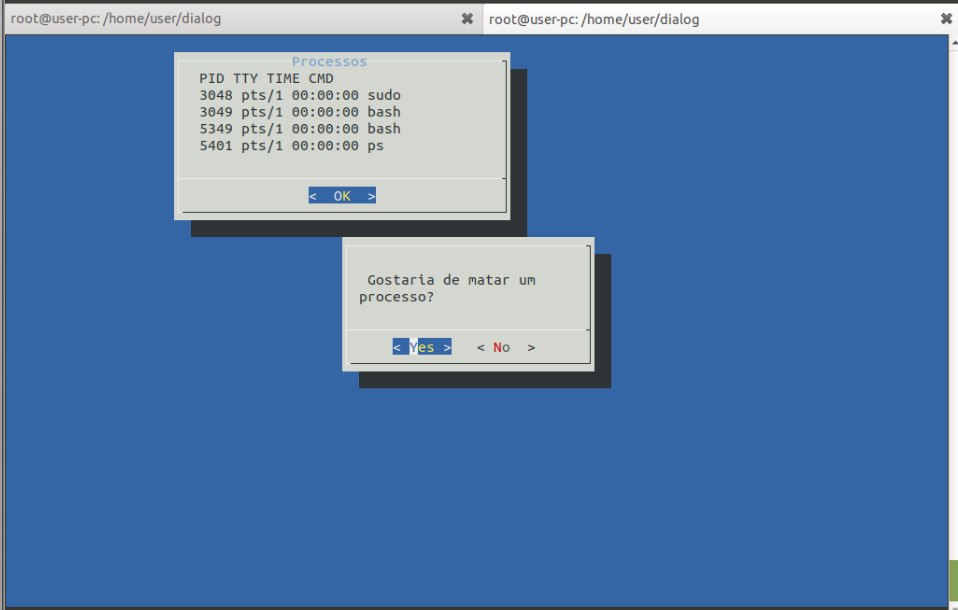
\includegraphics[width=1\linewidth]{fig/dialog/dialog10.png}
    \caption{Menu para matar um processo}
    \label{fig:dialog10}
\end{figure}

A interface também disponibiliza uma opção para consulta das configurações gerais do sistema operacional. Conforme apresentado na Figura \ref{fig:dialog11}, são exibidas informações como a versão do kernel, compilador utilizado e data da compilação. Essa funcionalidade permite ao administrador verificar rapidamente a versão do sistema em execução, facilitando atividades de manutenção, auditoria e diagnóstico do ambiente.


\begin{figure}[H]
    \centering
    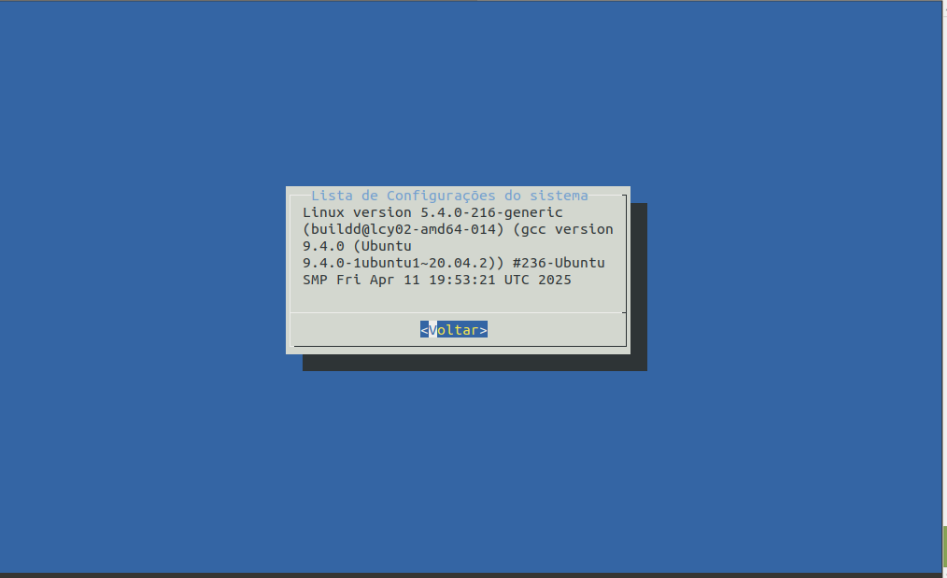
\includegraphics[width=1\linewidth]{fig/dialog/dialog11.png}
    \caption{Lista da configuração do sistema}
    \label{fig:dialog11}
\end{figure}

Para a realização dos testes de desempenho da rede utilizando o Iperf, foi desenvolvida uma interface específica para coleta dos parâmetros necessários. A Figura \ref{fig:dialog12} apresenta a tela de configuração inicial, na qual o usuário informa os dados do cliente e do servidor, incluindo nomes, endereços IP e credenciais de acesso. Essas informações são utilizadas pela aplicação para estabelecer a comunicação entre as máquinas virtuais participantes dos testes.


\begin{figure}[H]
    \centering
    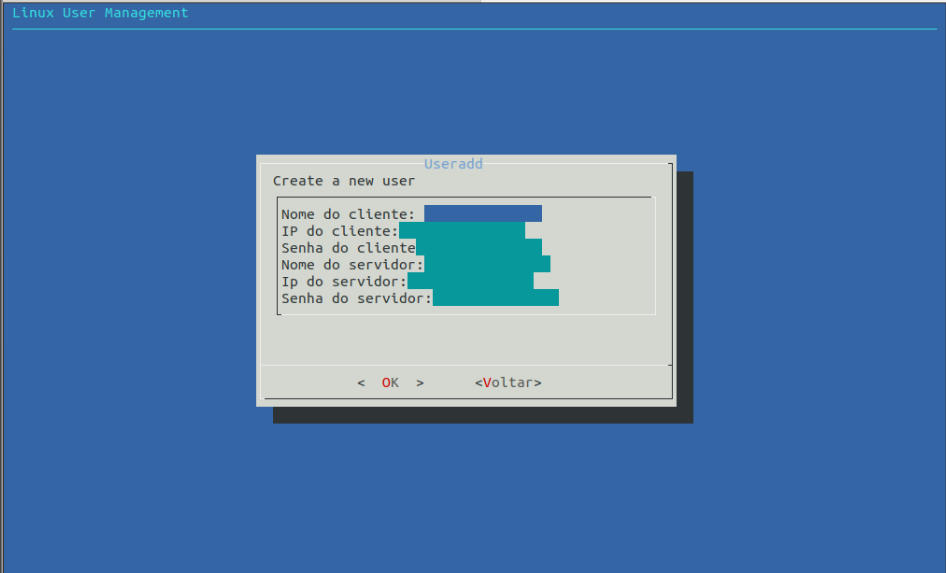
\includegraphics[width=1\linewidth]{fig/dialog/dialog12.png}
    \caption{Iperf 1}
    \label{fig:dialog12}
\end{figure}

Após o preenchimento dessas informações, é apresentada a tela ilustrada na Figura \ref{fig:dialog13}, responsável pela seleção do tipo de tráfego a ser gerado durante o teste. O usuário pode optar entre a transmissão de arquivos (\textit{Arquivo}) ou tráfego de voz (\textit{Voice}), possibilitando a avaliação do comportamento da rede em diferentes cenários de utilização. Essa abordagem permite automatizar a execução dos testes de desempenho sem a necessidade de inserir manualmente os comandos do Iperf em cada máquina virtual.

\begin{figure}[H]
    \centering
    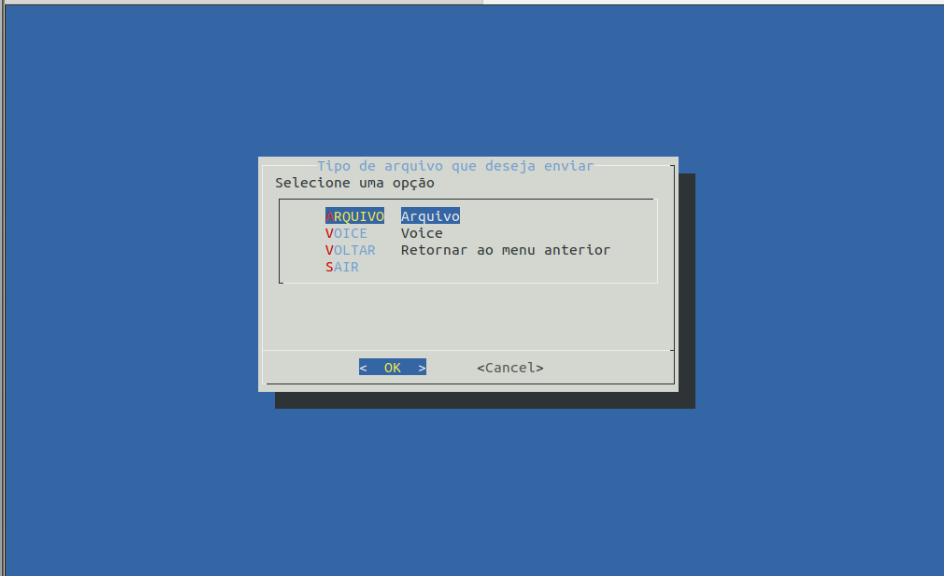
\includegraphics[width=1\linewidth]{fig/dialog/dialog13.png}
    \caption{Iperf - Seleção do tipo de arquivo a ser enviado}
    \label{fig:dialog13}
\end{figure}

As Figuras \ref{fig:dialog14}, \ref{fig:dialog15} e \ref{fig:dialog16} apresentam as telas de parametrização dos testes realizados com o Iperf. Após a escolha do tipo de tráfego, a interface solicita ao usuário os parâmetros específicos necessários para a execução do teste, permitindo configurar diferentes cenários de avaliação da rede.

A Figura \ref{fig:dialog14} corresponde à configuração do teste de transferência de arquivos. Nessa etapa podem ser definidos parâmetros como o número de conexões simultâneas, comprimento do buffer, tamanho máximo do segmento TCP (MSS), porta de comunicação, tamanho do buffer do socket, unidade utilizada para apresentação dos resultados e tempo de transmissão. Esses parâmetros possibilitam ajustar a intensidade do tráfego gerado e adequar os testes aos diferentes cenários de avaliação.


\begin{figure}[H]
    \centering
    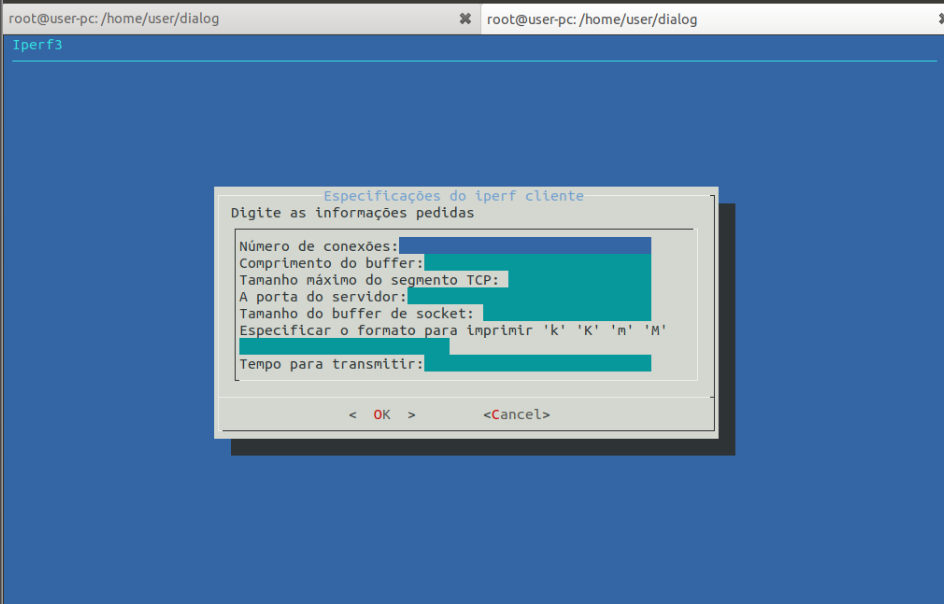
\includegraphics[width=1\linewidth]{fig/dialog/dialog14.png}
    \caption{Iperf - Informações do cliente Arquivo}
    \label{fig:dialog14}
\end{figure}


Para os testes de tráfego de voz, a interface apresenta telas específicas para o cliente e para o servidor. A Figura \ref{fig:dialog15} mostra a configuração do lado cliente, permitindo selecionar o protocolo de transporte (TCP ou UDP), definir o tamanho do segmento, largura de banda, número de conexões, unidade de exibição dos resultados, tamanho dos buffers e duração da transmissão. Esses parâmetros possibilitam simular aplicações de voz sobre IP (VoIP), cuja característica principal é a geração contínua de tráfego em tempo real.


\begin{figure}[H]
    \centering
    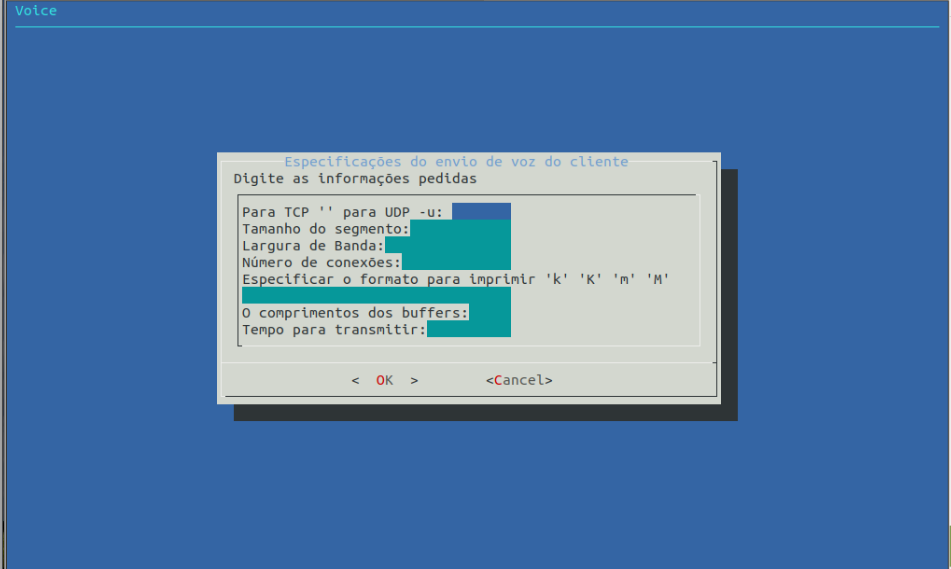
\includegraphics[width=1\linewidth]{fig/dialog/dialog15.png}
    \caption{Iperf - Informações do cliente  Voz}
    \label{fig:dialog15}
\end{figure}

Por sua vez, a Figura \ref{fig:dialog16} apresenta a configuração correspondente ao lado servidor do teste de voz. Nessa interface são definidos os parâmetros necessários para a inicialização do servidor Iperf, garantindo que ambos os extremos da comunicação utilizem configurações compatíveis durante a execução dos testes. Com isso, a ferramenta permite realizar avaliações de desempenho de forma padronizada, fornecendo informações relevantes para análise da largura de banda disponível, estabilidade da comunicação e comportamento da infraestrutura de rede sob diferentes condições de tráfego.


\begin{figure}[H]
    \centering
    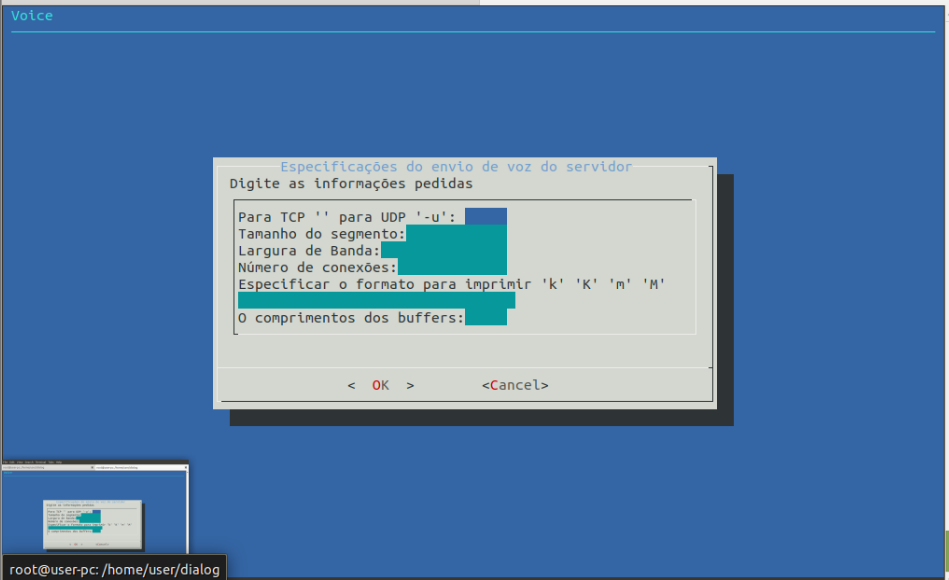
\includegraphics[width=1\linewidth]{fig/dialog/dialog16.png}
    \caption{Iperf - Informações do servidor  Voz}
    \label{fig:dialog16}
\end{figure}
